% Options for packages loaded elsewhere
\PassOptionsToPackage{unicode}{hyperref}
\PassOptionsToPackage{hyphens}{url}
%
\documentclass[
]{article}
\usepackage{amsmath,amssymb}
\usepackage{lmodern}
\usepackage{iftex}
\usepackage[a4paper, total={7in, 10in}]{geometry}
\ifPDFTeX
\usepackage[T1]{fontenc}
\usepackage[utf8]{inputenc}
\usepackage[english,russian]{babel}
  \usepackage{textcomp} % provide euro and other symbols
\else % if luatex or xetex
  \usepackage{unicode-math}
  \defaultfontfeatures{Scale=MatchLowercase}
  \defaultfontfeatures[\rmfamily]{Ligatures=TeX,Scale=1}
\fi
% Use upquote if available, for straight quotes in verbatim environments
\IfFileExists{upquote.sty}{\usepackage{upquote}}{}
\IfFileExists{microtype.sty}{% use microtype if available
  \usepackage[]{microtype}
  \UseMicrotypeSet[protrusion]{basicmath} % disable protrusion for tt fonts
}{}
\makeatletter
\@ifundefined{KOMAClassName}{% if non-KOMA class
  \IfFileExists{parskip.sty}{%
    \usepackage{parskip}
  }{% else
    \setlength{\parindent}{0pt}
    \setlength{\parskip}{6pt plus 2pt minus 1pt}}
}{% if KOMA class
  \KOMAoptions{parskip=half}}
\makeatother
\usepackage{xcolor}
\IfFileExists{xurl.sty}{\usepackage{xurl}}{} % add URL line breaks if available
\IfFileExists{bookmark.sty}{\usepackage{bookmark}}{\usepackage{hyperref}}
\hypersetup{
  hidelinks,
  pdfcreator={LaTeX via pandoc}}
\urlstyle{same} % disable monospaced font for URLs
\usepackage{graphicx}
\makeatletter
\def\maxwidth{\ifdim\Gin@nat@width>\linewidth\linewidth\else\Gin@nat@width\fi}
\def\maxheight{\ifdim\Gin@nat@height>\textheight\textheight\else\Gin@nat@height\fi}
\makeatother
% Scale images if necessary, so that they will not overflow the page
% margins by default, and it is still possible to overwrite the defaults
% using explicit options in \includegraphics[width, height, ...]{}
\setkeys{Gin}{width=\maxwidth,height=\maxheight,keepaspectratio}
% Set default figure placement to htbp
\makeatletter
\def\fps@figure{htbp}
\makeatother
\setlength{\emergencystretch}{3em} % prevent overfull lines
\providecommand{\tightlist}{%
  \setlength{\itemsep}{0pt}\setlength{\parskip}{0pt}}
\setcounter{secnumdepth}{-\maxdimen} % remove section numbering
\ifLuaTeX
  \usepackage{selnolig}  % disable illegal ligatures
\fi

\author{}
\date{}

\begin{document}
\begin{center}

\Huge
\textbf{Руководство пользователя~«3DViewer»}
\end{center}
\pagebreak[5]
\huge
\textbf{Содержание}
\LARGE
\begin{enumerate}
\def\labelenumi{\arabic{enumi}.}
\item
  \textbf{Введение........3}
\item
  \textbf{Загрузка модели..........4}
\item
  \textbf{Аффинные преобразования............5}
\item
  \textbf{Настройки
  модели\ldots\ldots.............6}
\item
  \textbf{Сохранение файлов............7}
\end{enumerate}
\pagebreak[5]
\huge
\textbf{Введение}
\newline
\LARGE
\begin{quote}
\textbf{3DViewer~---} это программа для просмотра 3D моделей в формате
\emph{\textbf{obj}}. Программа была разработана на операционной системе
MacOS 10.15 Catalina на языке программирования ``C''. Графический
интерфейс программы был создан с помощью приложения «QC Creator».
\newline
В \textbf{3DViewer}'е присутствует окно для отображения изображения 3D
модели. Программа позволяет в реальном времени изменять положение модели
относительно осей координат, вращать и масштабировать модель. Также
присутствуют различные настройки для изменения цвета, толщины линий и
размера вершин модели.
\end{quote}
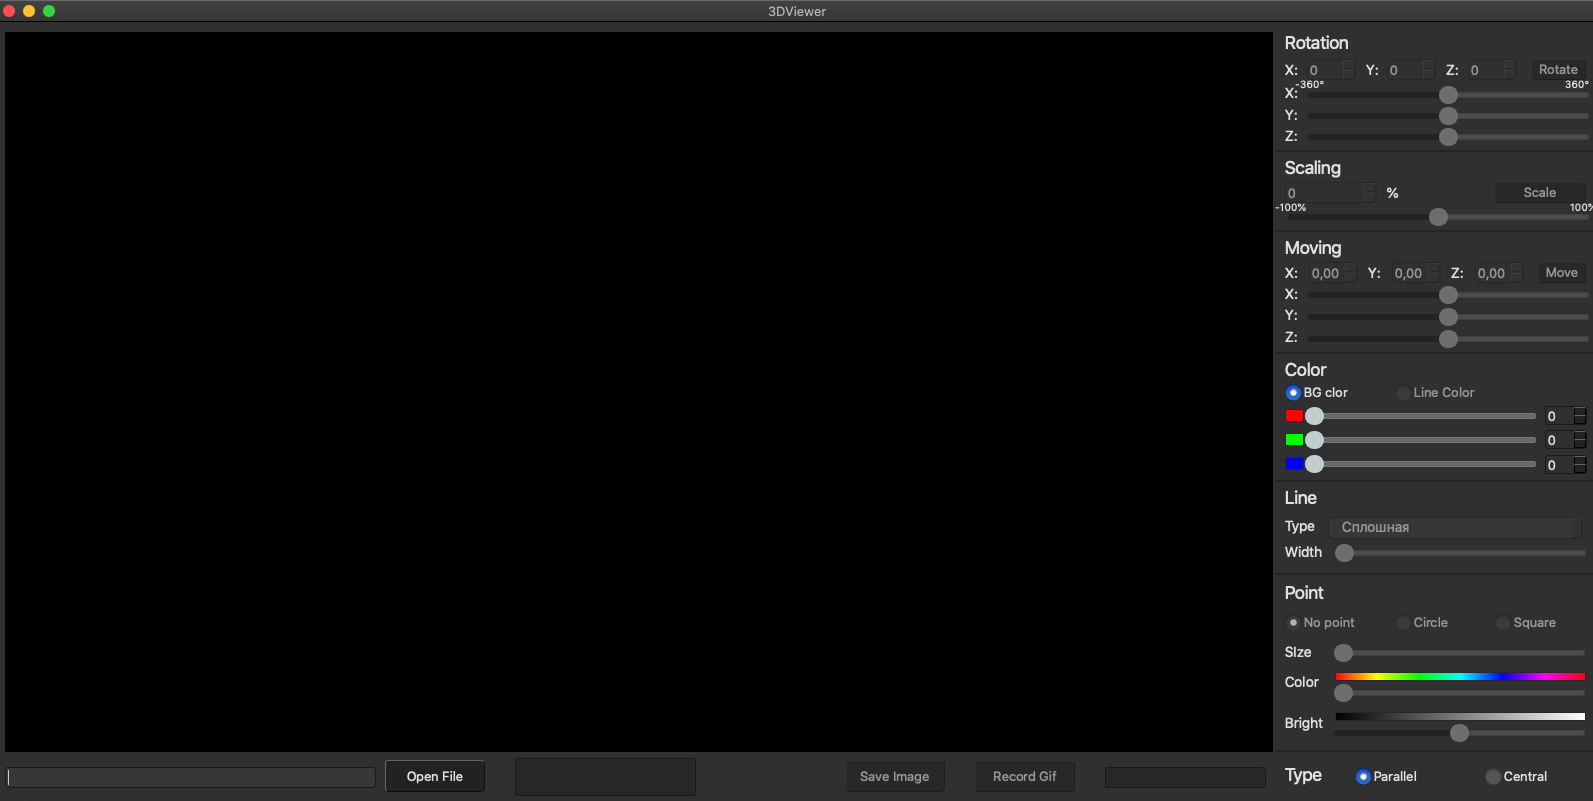
\includegraphics[bb=0 0 1200 650]{media/image1.png}
\pagebreak[15]

\huge
\textbf{Загрузка модели}
\newline
\LARGE
\begin{quote}
Чтобы загрузить модель, необходимо воспользоваться кнопкой \textbf{«Open
file»}, модель будет отображена в соответствующем окне, границы которого
задаются в зависимости от максимальных координат точек модели. Рядом с
кнопкой \textbf{«Open file»} отображается количество вершин и граней
модели. Название модели отображается над моделью на верхней рамке окна
приложения.
\end{quote}
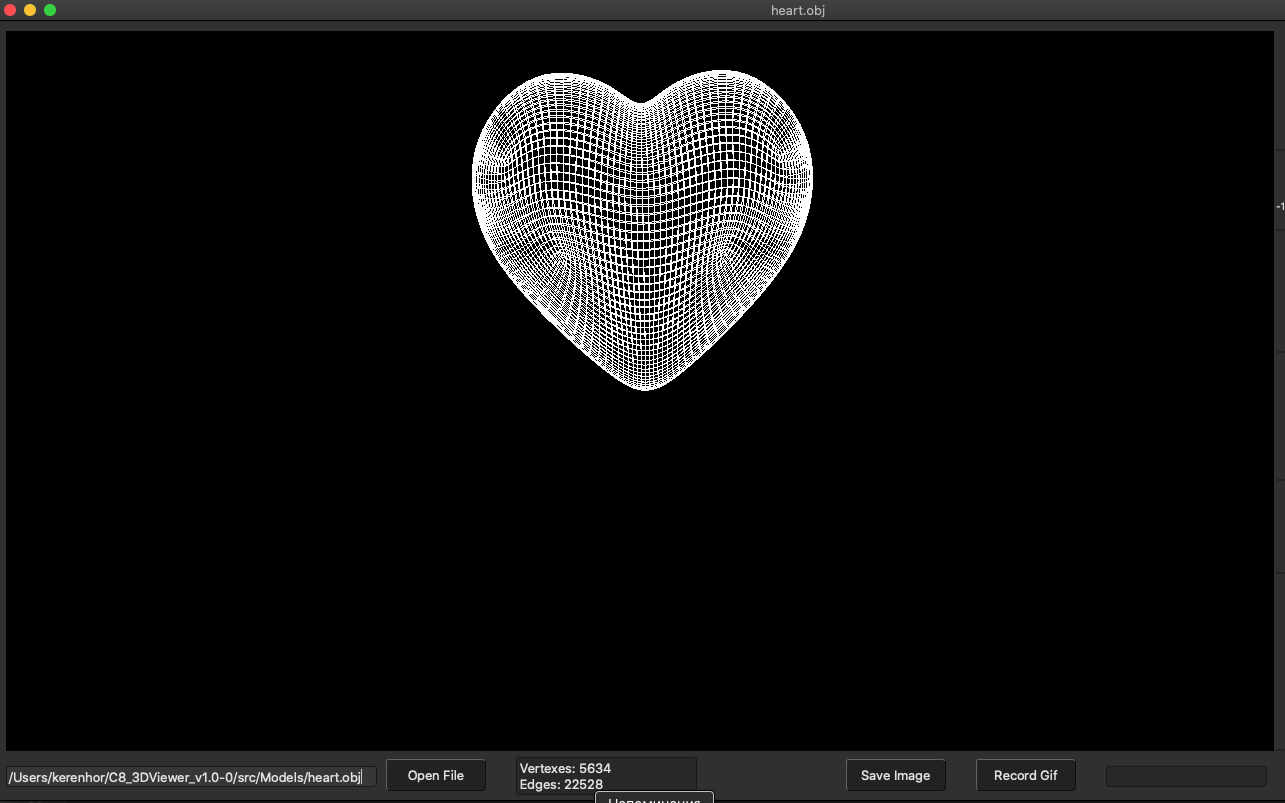
\includegraphics[bb=0 0 1000 650]{media/image2.png}
\pagebreak[25]

\huge
\textbf{Аффинные преобразования}
\newline
\LARGE
\begin{quote}
Справа от окна отображения модели находится панель для вращения,
масштабирования и изменения положения модели. Вращать, двигать и
масштабировать можно как с помощью слайдеров, так и вручную задавая
значения и нажимая на соответствующую кнопку.
\begin{center}
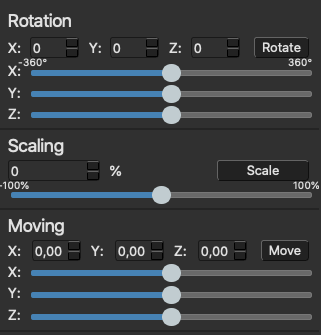
\includegraphics[bb=0 0 380 260]{media/image3.png}
\end{center}
\end{quote}
\pagebreak[30]
\huge
\textbf{Настройки модели}
\newline
\LARGE
\begin{quote}
Можно настроить формат отображения модели, а именно:
\end{quote}

\begin{itemize}
\item
  Цвет фона -- настраивается тремя слайдерами R, G, B.
\item
  Цвет линий -- выбираем «Line Color» и настраиваем аналогично цвету
  фона.
\item
  Линии -- доступно два типа линий: сплошная и пунктирная, с помощью
  слайдера настраивается ширина линий.
\item
  Вершины -- доступно три типа отображения вершин: без отображения,
  круглая точка, квадратная точка. Для изменения размера вершины
  используется слайдер. Для изменения цвета вершины есть два слайдера,
  один отвечает за цвет, второй за яркость.
\item
  Тип проекции -- есть два типа проекции на выбор: параллельная и
  центральная.
\end{itemize}

\begin{quote}
  \begin{center}
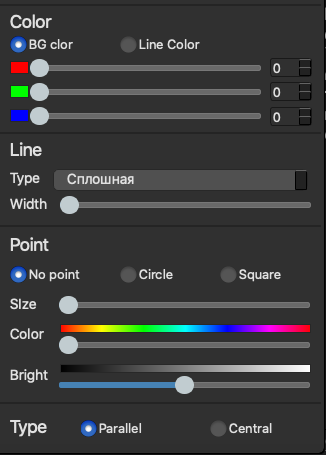
\includegraphics[bb=0 0 480 360]{media/image4.png}
  \end{center}
\end{quote}
\pagebreak[10]
\huge
\textbf{Сохранение файлов}
\newline
\LARGE
\begin{quote}
Для сохранения файлов под окном отображения модели имеется две кнопки:
\textbf{«Save Image»} и \textbf{«Record Gif»}.

\textbf{Save Image} -- позволяет сохранить текущее отображение модели в
форматах \emph{\textbf{.bmp}} и \emph{\textbf{.jpg}}.

\textbf{Record Gif} -- записывает анимированный gif-файл, когда
применяются аффинные преобразования. Справа от кнопки отображено
количество кадров(преобразований) до сохранения файла.
\end{quote}

\includegraphics[bb=0 0 180 60]{media/image5.png}
\end{document}
